\documentclass[conference,compsoc]{IEEEtran}
% Working paper draft using the IEEE conference layout. The venue and
% author block should be updated only after the manuscript is complete.
\IEEEoverridecommandlockouts

\usepackage{cite}
\usepackage{amsmath,amssymb,amsfonts}
\usepackage{algorithmic}
\usepackage{graphicx}
\usepackage{textcomp}
\usepackage{xcolor}
\usepackage{xspace}
\usepackage{hyperref}
\hypersetup{hidelinks}
\usepackage{tikz}
\usepackage{booktabs}
\usepackage{listings}
\usepackage{balance}
\usetikzlibrary{positioning}
\usetikzlibrary{shapes.geometric}
\usetikzlibrary{arrows.meta}

\newcommand{\toolname}{ParseRE\xspace}
\newcommand{\QEMU}{\textsc{QEMU}\xspace}

\lstset{
  basicstyle=\ttfamily\footnotesize,
  breaklines=true,
  columns=flexible,
  frame=single,
  numbers=left,
  numberstyle=\tiny\color{gray},
  keywordstyle=\color{blue},
  commentstyle=\color{green!50!black},
  stringstyle=\color{red!70!black},
}

\begin{document}

\title{Recovering Semantics from Unknown Binaries\\with Known Input Formats}

\author{
\IEEEauthorblockN{Anonymous}
\IEEEauthorblockA{Anonymous Institution}
}

\maketitle

\begin{abstract}
Reverse engineers who already understand the input format a binary parses spend most of their initial effort locating the code that implements each piece of the format.
We present \toolname, a binary-only tool that automates that step.
Given a grammar template for the input format, \toolname instantiates a corpus of structurally varied inputs, records \QEMU translation logs, compares pairs whose parse trees differ in exactly one production, and attributes differential trace-derived edges to that production.
A two-step uniqueness filter removes shared evidence, and the result is a trace-derived graph whose surviving records carry candidate grammar-rule labels.
The prototype requires neither source code nor compiler instrumentation, although its translation-log tracer does not capture a guaranteed complete dynamic execution sequence.
The artifact contains completed runs for Curl URI parsing, json-c, and libelf, plus planned evaluations for Apache APR and HPACK.
On the completed ELF evaluation against libelf, manual review yields 62 strict true positives among 68 labeled basic blocks (91.2\%), with one additional marginal case.
Accuracy review for the committed URI and JSON outputs remains future work.
\end{abstract}

\begin{IEEEkeywords}
reverse engineering, binary analysis, control-flow graphs, parser analysis, input format recovery, QEMU
\end{IEEEkeywords}

% ============================================================
\section{Introduction}\label{sec:intro}

At the outset of a reverse-engineering project, the engineer must develop a sense of the program's high-level behavior in order to identify points of interest that warrant careful analysis.
When the target's input format is well understood, much of that triage reduces to identifying which instructions in the binary implement which features of the input language.
This paper presents a technique for doing exactly that.
The basic idea is to run the target on a large corpus of valid inputs while collecting control flow traces, identify corpus elements with similar parse trees, and associate the delta in their control flow with the delta between their parse trees.

Consider a proprietary binary that validates TLS certificates.
The analyst knows the input is an X.509 certificate and understands its grammar (version fields, subject names, key material, extensions) but has no source code.
\toolname takes the certificate grammar together with a set of structurally varied certificates, traces the binary under \QEMU, and produces a labeled control-flow graph in which each grammar element maps to the basic blocks that process it.
The analyst then begins reverse engineering with a semantically meaningful map of the parser rather than raw disassembly.

We present \toolname and evaluate it on four input formats spanning the Chomsky hierarchy~\cite{chomsky1956three}: a regular language (URI), a context-free language (JSON), a context-sensitive binary format with internal compression (HPACK), and a structured offset-driven binary format (ELF).
For each format we run \toolname on one or more popular open-source implementations, then validate by manually checking that each labeled basic block implements the grammar rule indicated by its label.

\textbf{Contributions.} Our paper makes the following contributions to the field of reverse engineering:
\begin{itemize}
    \item We introduce the first binary-only technique that transfers semantic labels from program inputs onto control-flow graph edges and nodes. This bridges the gap between input formats and program internals, assisting reverse engineering and parser understanding (Section~\ref{sec:design}).
    \item We implement our technique in \toolname, a Python tool that requires only \QEMU and the target binary. We release \toolname as open source and demonstrate it on four input formats from different language classes (Section~\ref{sec:implementation}).
    \textit{[BEN: confirm we can publish the public repo URL in the camera-ready. For dual-blind we leave it anonymous.]}
    \item We evaluate \toolname on real-world parsers (Curl, Apache APR, json-c, libelf, and nghttp2) and validate every label through manual inspection (Section~\ref{sec:evaluation}).
    \item Our work lays the groundwork for future applications in differential fuzzing, grammar mining, and vulnerability discovery (Section~\ref{sec:future}).
\end{itemize}

\section{Background}\label{sec:background}

\subsection{Control-Flow Graphs}\label{sec:bg:cfg}

Reverse engineering is the process of analyzing a binary to understand its structure, functionality, and behavior without access to source code.
A fundamental program representation in this domain is the \textbf{control-flow graph (CFG)}.
Each node in a CFG corresponds to a \textbf{basic block}: a maximal sequence of consecutive instructions with a single entry point and a single exit point~\cite{shoshitaishvili2016sok}.
If execution reaches the first instruction of a basic block, it will execute every instruction in that block before transferring control elsewhere.
Edges in a CFG represent transfers of control flow, including branches, function calls, and returns.

Understanding how a program's input drives its execution path through the CFG is crucial to understanding the program's behavior.
For a parser binary, different inputs exercise different paths, and the structural differences between inputs correspond to structural differences in the paths taken through the parser code.

\subsection{Execution Tracing with QEMU}\label{sec:bg:qemu}

\QEMU~\cite{bellard2005qemu} is an open-source emulator that supports both full-system and user-mode emulation across many architectures.
In user-mode emulation, \QEMU executes a single Linux binary by translating its instructions and forwarding system calls to the host kernel.

A useful feature for binary analysis is \QEMU's logging facility, which records every basic block the emulator translates along with the block's start address and the disassembly of its first and last instructions.
This produces a complete, ordered basic-block trace of one program execution without any modification to the target binary.

This capability is central to our approach.
We trace the target under \QEMU for many inputs and compare the resulting traces to infer which code regions correspond to which input features.

\subsection{Parse Trees and Input Annotations}\label{sec:bg:parsetrees}

A \textbf{parse tree} represents the syntactic structure of an input according to a grammar.
Internal nodes correspond to grammar productions; leaves hold the concrete bytes.

We use parse trees to annotate inputs: each subtree is labeled with the grammar production it instantiates.
When two inputs share the same tree structure except at one subtree, the difference in their execution traces can be attributed to the differing production.
This is the core insight behind \toolname.

\section{Design}\label{sec:design}

\toolname runs as a four-stage pipeline, shown in Figure~\ref{fig:overview}.
The top row converts a grammar template into per-input translation logs.
The bottom row converts those logs into a labeled trace-derived graph.
Every stage except the grammar template itself is format-agnostic; adding a new format requires only writing a new template and compiling a small harness against the parser library under test.

\begin{figure*}[t]
\centering
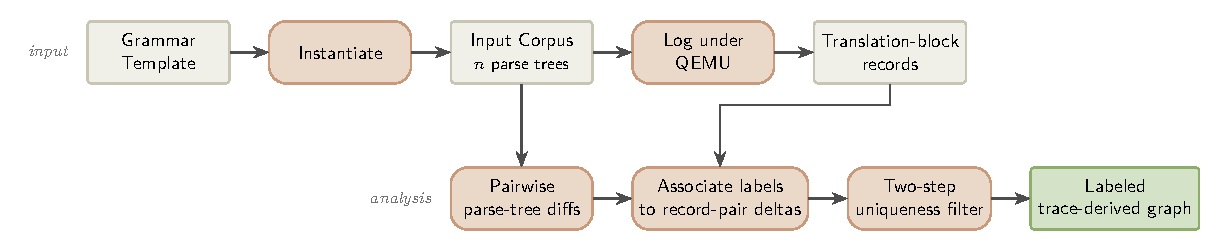
\includegraphics[width=0.92\linewidth]{figures/pipeline.pdf}
\caption{The \toolname pipeline. Cream rectangles are data artifacts. Salmon rounded rectangles are processing steps. The green rectangle is the final output. Vertical arrows bridge the two rows: the input corpus drives translation logging and pairwise input differencing, while the resulting block records feed label association.}
\label{fig:overview}
\end{figure*}

\subsection{Corpus Generation}\label{sec:design:corpus}

A grammar template is a tree of production rules.
Each leaf carries a small set of byte-level alternatives; each internal node carries a set of child configurations.
\toolname enumerates every combination of alternatives through Cartesian product, producing a corpus of concrete inputs each paired with its parse tree.

The templates are deliberately small.
The JSON template covers objects, arrays, strings, numbers, booleans, null, and a handful of degenerate cases (nan, inf), instantiating to 27 inputs.
The URI template covers scheme, authority, path, query, and fragment, instantiating to 1{,}458 inputs.
The ELF template, described in Section~\ref{sec:eval:elf}, instantiates to 20 inputs.

\textbf{The key property.}
For every pair of inputs we generate, the parse trees differ in either a single production or a small set of productions.
This is what makes attribution possible.
If two inputs differed in arbitrary ways, the trace differences between them could not be cleanly attributed to any single grammar element.

\subsection{Execution Tracing}\label{sec:design:trace}

Each input is fed to the target binary, which runs under \QEMU in user-mode emulation.
\QEMU logs translation blocks to a per-input file with each block's start address and disassembly.
\toolname parses the records into an ordered sequence, retains only blocks within the target binary's executable segment, and converts consecutive records into a trace-derived edge map.
These record pairs are useful differential signals, but the \texttt{-d in\_asm} translation log does not guarantee that every pair is a dynamic CFG edge.

Logs from inputs that the harness rejects (non-zero exit status) are dropped so the graph reflects only accepted corpus members.

\subsection{Label Association}\label{sec:design:assoc}

For every pair of inputs $(T_i, T_j)$ whose parse trees differ in exactly one production $p$, \toolname computes the consecutive-record-pair delta $E_i \setminus E_j$ and associates those pairs with $p$.
Aggregating over every input pair that isolates $p$ yields a per-production evidence set.

\textbf{Two-step uniqueness filter.}
Raw edge-to-label associations are noisy.
Many edges are shared across productions, including error-handling code and shared token-tape advancement.
\toolname strips this noise in two steps:

\begin{enumerate}
    \item \textbf{Subset removal.} If the edge set for production $p_1$ is nearly a subset of the edge set for $p_2$ ($|p_1 \setminus p_2| / |p_1| < 0.1$), \toolname removes $p_1$'s edges from $p_2$'s set. This eliminates setup and teardown code that runs for multiple productions but is most strongly associated with one.
    \item \textbf{Strict uniqueness.} For every production, \toolname subtracts the edges attributed to every other production. Edges that survive belong to a single production and receive its label.
\end{enumerate}

After filtering, \toolname propagates colors backward through the trace-derived graph.
A node whose outgoing edges all carry the same label is itself labeled with that color, which captures basic blocks that serve as sole entry points into a production-specific subgraph.

\subsection{Output}\label{sec:design:output}

\toolname emits three artifacts: a Graphviz DOT file of the labeled trace-derived graph, a rendered SVG for browser inspection, and an address-to-label mapping.
The mapping can be adapted for import into a disassembler, but this artifact does not yet include a dedicated import script.

\section{Implementation}\label{sec:implementation}

\toolname is implemented as a single Python module with minimal external dependencies and parallelized across available CPU cores using a thread pool.
The tool requires Python and \QEMU user-mode emulation; the analyst supplies the target binary and a grammar template for the input format.

\subsection{Corpus Generation}\label{sec:impl:corpus}

Grammar templates are written as nested tree structures.
Each template node has a name (the grammar production) and a set of alternatives, which are either concrete byte sequences at leaf nodes or sets of child configurations at internal nodes.
\toolname recursively enumerates every combination of alternatives via Cartesian product, producing a set of concrete parse trees that can be serialized to byte strings.

For JSON, the template covers seven productions: object, string, number, boolean, null, nan, inf, and array, with multiple byte-level alternatives for each.
For URI, it covers scheme, authority (with optional userinfo, host, and port), path, query, and fragment.
Adding a new format requires only defining a new template and a corresponding harness binary; no changes to the core pipeline are needed.

The number of instantiations a template produces depends on its branching factor.
The JSON template yields 27 instantiations (729 pairwise comparisons), the URI template yields 1{,}458 instantiations (over two million pairwise comparisons), and the ELF template yields 20 instantiations (380 pairwise comparisons).
Each input is small (under one kilobyte for the text formats; exactly 1048 bytes for ELF), which keeps trace collection practical even for large corpora.

\subsection{Tracing with QEMU}\label{sec:impl:qemu}

Each input is fed to the target binary via standard input.
\toolname invokes \QEMU in user mode with logging enabled and a per-input output file.
The target is a small harness that reads from standard input, calls the parser library under test, and exits with a status code indicating parse success or failure.

After execution, \toolname parses the trace file with a regular expression that extracts basic-block boundaries from the \QEMU log.
Each record contains the block's start address and the addresses of its first and last instructions, from which the tool constructs a record for the basic block.
Only blocks within the target binary's executable segment are retained; blocks from the dynamic linker and the \QEMU runtime are discarded.

Traces for inputs that the parser rejects (non-zero exit status) are excluded from subsequent analysis.
This ensures the CFG is built from successful parses, where the parser exercises its full grammar-handling logic.

\textit{[BEN: the trace-log regex is version-dependent. Worth confirming it is robust across the QEMU versions we expect reviewers to use, or pinning the version in the artifact description.]}

\subsection{Target Harnesses}\label{sec:impl:harness}

For each parser under test, we compile a small C harness that links against the parser library, reads input from standard input, invokes the top-level parse function, and returns the result.
Harnesses are typically under thirty lines of C, with the exception of the ELF harness, which walks the program header table, section header table, and symbol table explicitly to ensure each structure is exercised.

Harnesses are compiled inside Docker containers for reproducibility, and parser libraries are linked statically to keep dynamic-linker code out of the traces.
We compile at low optimization with inlining disabled (\texttt{-O0 -fno-inline}) so the compiler does not collapse distinct parser functions into inlined code, which would destroy the correspondence between grammar productions and basic-block ranges.
For evaluation purposes, harnesses also include debug information so that addresses can be resolved back to source lines via \texttt{addr2line}; this is helpful for manual verification but unnecessary for the core analysis.

\subsection{Supported Formats}\label{sec:impl:formats}

The current implementation includes grammar templates for four formats:

\begin{itemize}
    \item \textbf{URI} (regular): scheme, authority (userinfo, host, port), path, query, fragment, per RFC~3986.
    \item \textbf{JSON} (context-free): objects, arrays, strings, numbers, booleans, null, per RFC~8259.
    \item \textbf{HPACK} (context-sensitive binary): indexed headers, literal headers with and without Huffman compression, per RFC~7541.
    \textit{[BEN: fill in your HPACK template description when ready.]}
    \item \textbf{ELF} (offset-driven binary): a fixed ELF header, four program header variants that change the second segment type, and five section variants that change which sections are populated. Each instantiation is a valid 1048-byte ELF64 file produced by a generator script.
\end{itemize}

\section{Evaluation}\label{sec:evaluation}

The current artifact contains completed runs for three format-parser pairs: URI with Curl, JSON with json-c, and ELF with libelf.
Manual per-block review is complete for ELF; URI and JSON results are descriptive counts from the committed outputs.
Apache APR and HPACK are retained as planned extensions, not completed evaluations.

\textbf{Research questions.}
\begin{itemize}
    \item[\textbf{(Q1)}] How many basic blocks does \toolname label, and what fraction of the trace-derived graph do those labels cover?
    \item[\textbf{(Q2)}] For the reviewed ELF output, how accurate are the labels at the per-block level?
    \item[\textbf{(Q3)}] What preliminary differences appear across the three completed format-parser runs?
\end{itemize}

\subsection{Methodology}\label{sec:eval:method}

For each completed format-parser pair, we (1)~compile a harness against the parser library inside a Docker container with debug symbols and static linkage, and (2)~run \toolname with the corresponding grammar template under \QEMU user-mode.
For ELF, a human evaluator additionally checks each production-labeled block against the source location recovered via \texttt{addr2line} and classifies it as a strict true positive, false positive, or marginal case.
Because the evaluation does not enumerate all semantically relevant parser blocks independently of \toolname, it does not measure false negatives.

\textbf{Why manual inspection.}
Automated semantic verification without ground truth can introduce circularity or unsupported judgments.
Accordingly, the ELF accuracy result comes from manual inspection of the labeled graph, source mappings, and relevant parser routines.
URI and JSON accuracy values are intentionally left unreported until the same review is complete.

\subsection{URI Parsers}\label{sec:eval:url}

The completed URI run targets Curl's \texttt{curl\_url\_set}; a run against Apache Portable Runtime's \texttt{apr\_uri\_parse} remains planned.
The URI template instantiates 1{,}458 inputs and produces 2{,}124{,}306 ordered comparisons between distinct inputs.

\textbf{Curl.}
On the statically linked Curl harness, \toolname produces a trace-derived graph with 522 nodes and 558 edges.
The committed mapping contains 191 production-labeled blocks across 10 exact label strings and 21 blocks with the ambiguous \texttt{None} label.
Table~\ref{tab:url-labels} shows the distribution.
Host validation dominates because Curl's parser performs extensive checks: IPv4 versus IPv6 detection, IDNA processing, bracket handling, and length validation.
The duplicate-looking labels (\texttt{port} versus \texttt{:port}, \texttt{query} versus \texttt{?query}) come from the template's leaf naming: the colon or question mark delimiter is included in the label string. This is a template quirk; the underlying attribution is correct.

\begin{table}[h]
\caption{URI label distribution (Curl).}
\label{tab:url-labels}
\centering
\begin{tabular}{lr}
\toprule
Production & Labeled BBs \\
\midrule
host        & 91 \\
port        & 34 \\
segment     & 30 \\
userinfo    & 25 \\
query       & 5  \\
fragment    & 5  \\
path        & 1  \\
\textit{ambiguous} & 21 \\
\bottomrule
\end{tabular}
\end{table}

The 21 ambiguous blocks are code paths that the current filtering could not uniquely attribute to a single production.
Per-block accuracy has not yet been reviewed.

\textbf{Apache APR.}
The repository documents this as a planned replication with the same URI template, but it contains no APR output from which to report results.

\subsection{JSON Parsers}\label{sec:eval:json}

We evaluate on json-c, a widely deployed C library for JSON parsing.
The JSON template instantiates 27 inputs and produces 702 ordered comparisons between distinct inputs.

On json-c (commit \texttt{894856}), \toolname produces a trace-derived graph with 464 nodes and 400 edges, of which 295 basic blocks receive production labels across 6 productions.
Table~\ref{tab:json-labels} shows the distribution.

\begin{table}[h]
\caption{JSON label distribution (json-c).}
\label{tab:json-labels}
\centering
\begin{tabular}{lr}
\toprule
Production & Labeled BBs \\
\midrule
number         & 110 \\
object-element & 77  \\
string         & 39  \\
array          & 36  \\
boolean        & 24  \\
nan            & 9   \\
\bottomrule
\end{tabular}
\end{table}

\texttt{number} dominates because C-level numeric parsing is complex: sign handling, decimal point, exponent notation, overflow checks, and \texttt{strtod} wrappers each require their own basic blocks.
\texttt{nan} receives few labels because the parsing path is a three-character string comparison.

Per-block accuracy has not yet been reviewed for this output.

\subsection{HPACK Decoder}\label{sec:eval:hpack}

HPACK is the header compression format for HTTP/2, defined in RFC~7541~\cite{rfc7541}.
The format is fully binary, uses context-sensitive encoding, and includes a fixed Huffman table baked into the specification.
This would make HPACK a useful stress test for \toolname: it has binary encodings and conditional logic that text formats lack.
The planned target is nghttp2's HPACK decoder, but the repository does not yet contain a template or output for this evaluation.

\subsection{ELF Parser}\label{sec:eval:elf}

ELF is the standard binary format on Linux and other Unix-like systems.
Unlike the sequential text formats above, ELF is offset-driven: the ELF header contains pointers to program header and section header tables, which in turn point to string tables, symbol tables, and other sections.
We target libelf from elfutils, a widely used library for accessing ELF files.

\textbf{Corpus layout.}
Figure~\ref{fig:elf-layout} shows the layout of a single corpus instantiation.
Every corpus member is exactly 1{,}048 bytes with identical offsets, and varies only in three regions: the ELF header (one variant), the two-entry program header table (four variants that change the second program header's type field across \texttt{PT\_NOTE}, \texttt{PT\_INTERP}, \texttt{PT\_DYNAMIC}, and \texttt{PT\_NULL}), and the section region (five variants that toggle which sections contain real data versus zeroed bytes).
The Cartesian product yields $1 \times 4 \times 5 = 20$ instantiations and 380 pairwise comparisons.

\begin{figure}[t]
\centering
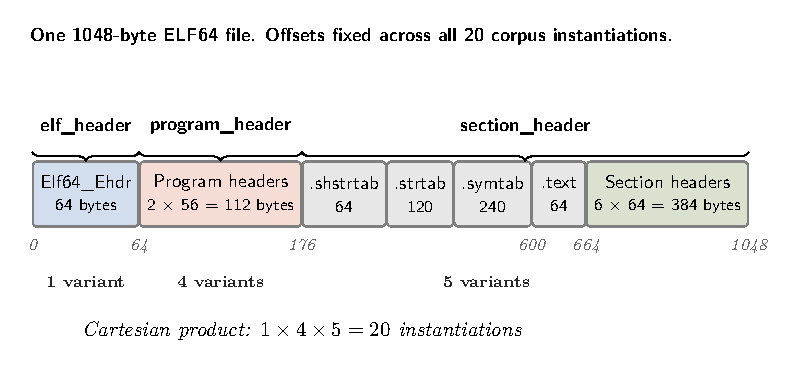
\includegraphics[width=\linewidth]{figures/elf-layout.pdf}
\caption{Fixed-layout ELF corpus. Every one of the 20 instantiations has the same byte offsets. The three template children (\texttt{elf\_header}, \texttt{program\_header}, \texttt{section\_header}) carry 1, 4, and 5 alternatives respectively.}
\label{fig:elf-layout}
\end{figure}

\textbf{Results.}
On libelf, \toolname produces a labeled trace-derived graph with 358 nodes and 354 record-pair edges.
Of these, 68 basic blocks receive the \texttt{section\_header} label.
The \texttt{program\_header} production receives zero labels despite having four template variants.

\textbf{Why \texttt{program\_header} is unlabeled.}
Libelf reads all program-header types through the same code path.
The \texttt{p\_type} field is data stored in a struct; libelf does not branch on it during parsing.
The retained translation-log evidence through \texttt{gelf\_getphdr} is therefore identical across the four variants, and the difference algorithm has no record pairs to attribute.
Section types, by contrast, do trigger different code paths: sections with \texttt{SHT\_SYMTAB} type cause the harness to iterate symbol entries via \texttt{gelf\_getsym} and resolve names via \texttt{elf\_strptr}, while null sections skip these operations.

\begin{table}[h]
\caption{ELF label distribution (libelf). The high ambiguity rate reflects libelf's structure: most code is shared across section types.}
\label{tab:elf-labels}
\centering
\begin{tabular}{lr}
\toprule
Production & Labeled BBs \\
\midrule
section\_header & 68 \\
\textit{ambiguous} & 202 \\
\bottomrule
\end{tabular}
\end{table}

\textbf{Where the labels land.}
Figure~\ref{fig:elf-cfg} shows 12 of the 68 labeled blocks, taken directly from our \texttt{out.dot}.
They cluster in three places: the harness's \texttt{walk\_section\_headers} loop, libelf's \texttt{\_\_libelf\_set\_rawdata\_wrlock} section-data initialization routine, and libelf's lookup routines (\texttt{elf\_strptr}, \texttt{gelf\_getsym}).
The cross-function arrows are consecutive records in the QEMU translation log: the corresponding paths appear when the harness reaches libelf's section setup and symbol-table walk for sections that carry a symbol table.

\begin{figure}[t]
\centering
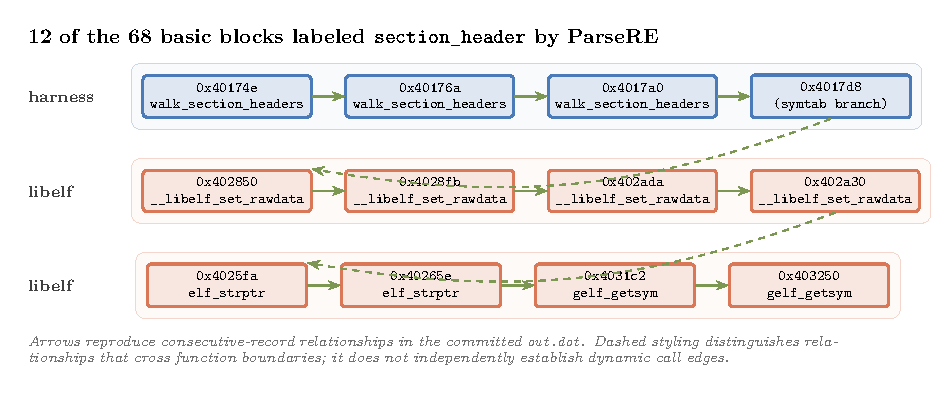
\includegraphics[width=\linewidth]{figures/elf-cfg-fragment.pdf}
\caption{12 of the 68 \texttt{section\_header}-labeled basic blocks. Arrows reproduce consecutive-record relationships from the committed trace-derived graph; dashed styling distinguishes relationships that cross function boundaries.}
\label{fig:elf-cfg}
\end{figure}

\textbf{Accuracy.}
Manual inspection of all 68 labeled blocks yields 62 strict true positives (91.2\%), 5 false positives, and 1 marginal case.
The 5 false positives all sit inside \texttt{\_\_gelf\_getehdr\_rdlock}, an ELF-header validation routine that libelf calls internally during section traversal.
Those blocks process the ELF header rather than section headers, but they are reached only through section-handling code paths and so appear in the differential edge set.
The review did not measure false negatives because it did not independently enumerate every block that should receive a grammar label.

\textbf{What this reveals about binary formats.}
The text-format runs produce 6 JSON label strings and 10 exact URI label strings, while the ELF run produces one (\texttt{section\_header}).
This result is consistent with the tested libelf harness using uniform record readers for many structures and conditional consumer code for section and symbol-table handling.
It should not yet be generalized to binary parsers as a class from one evaluated target.

\subsection{Cross-Format Comparison}\label{sec:eval:comparison}

\begin{table}[t]
\caption{Cross-format artifact summary. Inst.\ = template instantiations; BBs = total blocks in the trace-derived graph; Labels = production-labeled blocks; Acc.\ = strict true positives divided by all production-labeled blocks.}
\label{tab:crossformat}
\centering
\begin{tabular}{llrrrr}
\toprule
Format & Parser & Inst. & BBs & Labels & Acc.(\%) \\
\midrule
URI    & Curl          & 1{,}458  & 522  & 191  & -- \\
URI    & Apache APR    & 1{,}458  & --   & --   & -- \\
JSON   & json-c        & 27       & 464  & 295  & -- \\
HPACK  & nghttp2       & --       & --   & --   & -- \\
ELF    & libelf        & 20       & 358  & 68   & 91.2 \\
\bottomrule
\end{tabular}
\end{table}

\textbf{Coverage is not a function of corpus size.}
JSON uses 27 instantiations and labels 295 blocks (63.6\% of the graph).
URI uses 1{,}458 instantiations and labels 191 blocks (36.6\%), with 21 additional ambiguous records.
ELF uses 20 instantiations and labels 68 blocks (19\%).
These three observations show that a larger corpus does not automatically yield a higher labeling rate.
More formats, parsers, and reviewed outputs are required before attributing the differences to a format class or parser architecture.

\section{Related Work}\label{sec:rel}

\toolname occupies a specific niche in the binary-analysis landscape: it associates \textit{known} input-format labels with a binary's basic blocks using differential QEMU translation logs.
We position it against three lines of prior work that are easily confused with each other but solve materially different problems.

\subsection{Trace-Diffing Tools}\label{sec:rel:tenet}

Tenet~\cite{gaasedelen2021tenet} and Lighthouse~\cite{gaasedelen2017lighthouse} are disassembler plugins that highlight the basic blocks differing between execution traces of the same binary inside IDA~Pro or Binary~Ninja.
They are widely used in practice for tasks like identifying why one input crashes while another does not.

These tools solve a degenerate case of \toolname's problem: $N{=}2$ inputs, no input-side annotations.
\toolname generalizes the differential approach in two ways.
First, we systematically generate large corpora of structurally related inputs from a grammar template (Section~\ref{sec:design:corpus}) rather than asking the user to supply two interesting inputs by hand.
Second, we attach semantic labels to the input structure and propagate those labels to trace-derived record pairs, producing a format-aware annotation rather than a binary ``differs / does not differ'' verdict.

\subsection{Input-Region Categorization}\label{sec:rel:polyfile}

PolyFile~\cite{sultanik2019polyfile} from Trail of Bits identifies which byte ranges of a file belong to which substructure of a known file format.
PolyTracker~\cite{sultanik2024polytracker} extends this with whole-input dynamic information flow tracking, using LLVM instrumentation to build a directed acyclic graph that maps each input byte through the program's execution.

\toolname and these tools both operate on inputs whose formats are known, but they differ in what they annotate.
PolyFile produces an annotation of the \textit{input}.
PolyTracker produces a data-flow mapping between input bytes and program operations.
\toolname produces candidate annotations for binary locations represented in its trace-derived graph.
The three tools are therefore composable: PolyFile can produce the labeled corpus that \toolname consumes, and \toolname's output can be cross-referenced with PolyTracker's data-flow graph for deeper understanding.

A methodological distinction separates \toolname from PolyTracker: PolyTracker uses LLVM-level instrumentation, whereas \toolname observes an executable through \QEMU user-mode emulation.
The resulting tradeoff is between richer byte-level data flow and a lighter-weight workflow that can be applied when a runnable binary and compatible emulation environment are available.

\subsection{Grammar Mining and Format Recovery}\label{sec:rel:grammar}

A substantial body of academic work addresses the inverse problem: given only a binary, recover the grammar of the inputs it accepts.
Tupni~\cite{cui2008tupni} performs automatic reverse engineering of input formats using dynamic analysis.
Polyglot~\cite{caballero2007polyglot} extracts protocol message formats via dynamic binary analysis.
AUTOGRAM~\cite{hoschele2016autogram} infers grammars from observed input-output behavior using dynamic taint analysis.
More recent work by Gopinath et~al.~\cite{gopinath2020mining} mines context-free input grammars from dynamic control flow.
Prospex~\cite{comparetti2009prospex} recovers protocol state machines from network traces.

These approaches answer the question \textit{``what does this binary eat?''}
\toolname answers a different question: \textit{``given that this binary eats X, where in the code is X handled?''}
The two problems are sequential rather than competing.
An analyst would use a grammar-recovery tool to obtain a starting grammar, then use \toolname to map that grammar onto the code.
Conflating the two would be a category error.

A second methodological distinction concerns observation cost and evidence.
Grammar-recovery systems span compiler instrumentation, dynamic taint analysis, and binary-level execution analysis; several, including Tupni and Polyglot, operate directly on binaries.
\toolname does not recover an unknown grammar or track byte-level data flow.
It instead assumes a known template and uses lightweight \QEMU translation-log differences, trading semantic depth for easier deployment on compatible runnable binaries.

\subsection{Differential Testing for Parsers}\label{sec:rel:difftesting}

The broader idea of detecting parser bugs through differential observation has been explored in the HTTP/1.1 ecosystem~\cite{http-smuggling} and in static differential analysis of protocol parsers~\cite{zheng2024pardiff}.
These tools surface discrepancies in protocol semantics between parser implementations.
\toolname surfaces the structural correspondence between an agreed input grammar and the code that realizes it.
They are complementary: a differential-testing tool can find that two parsers disagree, then \toolname can localize where in each parser the disagreement lives.

% TODO: Revisit the differential-parser citation set before publication.

\section{Future Work}\label{sec:future}

\textbf{Additional architectures.}
\toolname currently targets x86-64 binaries.
\QEMU supports many additional architectures (ARM, MIPS, RISC-V, PowerPC), and the only architecture-dependent component is the trace-log parser.
Extending to other architectures requires adapting the regular expression that extracts basic-block boundaries from \QEMU's log output.

\textbf{Differential fuzzing guided by labels.}
Once \toolname has labeled a parser's CFG, the labels provide a natural coverage metric for format-aware fuzzing.
A fuzzer could prioritize inputs that exercise under-explored grammar productions, using \toolname's labels as a coverage map.

\textbf{Grammar mining integration.}
As discussed in Section~\ref{sec:rel:grammar}, grammar-recovery tools and \toolname solve complementary problems.
An integrated pipeline could first recover an approximate grammar from a binary, then use \toolname to validate and refine the mapping, closing the loop between ``what does this binary eat?'' and ``where does it eat it?''

\textbf{Hierarchical labeling.}
The current template system supports one level of production-to-label mapping.
Extending to hierarchical templates (labeling not just ``string'' but ``string-escape-sequence'' versus ``string-literal-characters'') would increase the granularity of the output without algorithmic changes.

\section{Ethical Considerations}\label{sec:ethics}

\toolname is a defensive reverse-engineering tool that annotates binary code with format-semantic labels.
It does not discover, create, or exploit vulnerabilities.
All evaluated targets are publicly available software projects; the artifact contains no proprietary or classified binaries.
The present repository does not include a license file, so it should be treated as source-available for research review rather than as a licensed open-source release.

\section{LLM Usage Statement}\label{sec:llm}

Large language models were used for editorial assistance and exploratory checks while preparing this draft.
The committed ELF label counts reported here were manually reviewed; no unverified model-generated measurement is presented as a final result.

\section{Conclusion}\label{sec:conclusion}

We presented \toolname, a technique for associating known input-format labels with locations in an unknown binary.
By systematically generating structurally varied inputs, recording their \QEMU translation logs, and associating record-pair deltas with parse-tree deltas, \toolname produces candidate semantic annotations without requiring source code, compiler instrumentation, or data-flow analysis.

The artifact contains completed runs for URI, JSON, and ELF; manual validation is complete only for ELF, where 62 of 68 labels are strict true positives and one additional label is marginal.
These results support continued study, but broader accuracy claims require review of the URI and JSON outputs, completion of the planned APR and HPACK runs, and replacement or validation of the translation-log tracer with dynamic execution events.

% ============================================================

% TODO: Add contributor, advising, and funding acknowledgments after the
% author list and publication venue are settled.

\balance
\bibliographystyle{IEEEtran}
\bibliography{references}

\end{document}
